% ОБЯЗАТЕЛЬНО ИМЕННО ТАКОЙ documentclass!
% (Основной кегль = 14pt, поэтому необходим extsizes)
% Формат, разумеется, А4
% article потому что стандарт не подразумевает разделов
% Глава = section, Параграф = subsection
% (понятия "глава" и "параграф" из стандарта)
\documentclass[a4paper,article,14pt]{extarticle}

% Подключаем главный пакет со всем необходимым
\usepackage{spbudiploma}

% Пакеты по желанию (самые распространенные)
% Хитрые мат. символы
\usepackage{euscript}
% Таблицы
\usepackage{longtable}
\usepackage{makecell}
% Картинки (можно встявлять даже pdf)
\usepackage[pdftex]{graphicx}

\usepackage{amsthm,amssymb, amsmath}
\usepackage{textcomp}
\usepackage{amsmath}
\usepackage{comment}


\begin{document}

% Титульник в файле titlepage.tex
% --------------------- Стандарт СПбГУ для ВКР --------------------------
% Автор: Тоскин Николай, itonik@me.com
% Если заметили ошибку, напишите на email
% Если хотите добавить изменение самостоятельно, GitHub: . PR-s welcome!
% Использованы материалы:
% habr.com/ru/post/144648/
% cpsconf.ru
% Текст:
% http://edu.spbu.ru/images/data/normativ_acts/local/20181030_10432_1.pdf
% Титульный лист:
% http://edu.spbu.ru/images/data/normativ_acts/local/20180703_6616_1.pdf
% -----------------------------------------------------------------------

% Титульный лист диплома СПбГУ
% Временное удаление foot на titlepage
\newgeometry{left=30mm, top=20mm, right=15mm, bottom=20mm, nohead, nofoot}
\begin{titlepage}
\begin{center}
% Первый символ съедается, первым знаком поставлен Ы
\textbf{Санкт--Петербургский}
\textbf{государственный университет}

\vspace{35mm}

\textbf{\textit{\large Ковалев Святослав Сергеевич}} \\[8mm]
% Название
\textbf{\large Выпускная квалификационная работа}\\[3mm]
\textbf{\textit{\large Прогнозирование временных рядов методами машинного обучения}}

\vspace{20mm}
% TODO: Узнать как правильно
Уровень образования: бакалавриат\\
Направление 01.03.02 «Прикладная математика и информатика»\\
«Прикладная математика, фундаментальная информатика и программирование»\\


% Научный руководитель, рецензент
% Сходить в уч отдел и узнать, правильно ли
\begin{flushright}
{Научный руководитель:} \\
% TODO: Узнать кафедру
профессор, кафедра компьютерных технологий \\ и систем, д.ф. - м.н.  Буре~Владимир Мансурович
\end{flushright}
\begin{flushright}
{Рецензент:} \\
% TODO: Узнать кафедру
профессор, кафедра компьютерных технологий \\и систем, д.ф. - м.н.  Буре~Владимир Мансурович
\end{flushright}

\vfill 

{Санкт-Петербург}
\par{2020 г.}
\end{center}
\end{titlepage}
% Возвращаем настройки geometry обратно (то, что объявлено в преамбуле)
\restoregeometry
% Добавляем 1 к счетчику страниц ПОСЛЕ titlepage, чтобы исключить 
% влияние titlepage environment
\addtocounter{page}{1}

% Содержание
\tableofcontents
\pagebreak
\specialsection{Введение}
\documentclass[12pt]{article}
\begin{document}
Hello world!
$Hello world!$ %math mode
\end{document}

Ежедневно на Санкт-Петербургской международной товарно-сырьевой бирже\cite{spimex} ведутся торги различным сырьем: нефтепродукты, нефть, газ, электроэнергия и~т.\,д.
Торги идут сессиями фиксированной длины в каждый будний день. По результатам каждой торговой сессии публикуется отчет с информацией: средневзвешенная цена, лучшая заявка на покупку и продажу, общий объем продаж и другие показатели.
В данной работе рассмотрим прогнозирование средневзвешенной цены по нефтепродуктам на $n$ дней вперед по двум базисам поставки.

\specialsection{Еще одно введение}

Прогнозирование временных рядов - одна из главных задач в экономике и финансах.
Хотя эта задача достаточно изучена для определенного класса временных рядов, остаются нерешенные проблемы.
Например, прогнозирование цен биржевых торгов.
\par
Прогнозирование биржевых цен позволяет крупным компаниям принимать стратегические решения, а частным трейдерам совершать выгодные сделки.
Цель этой работы - показать эффективность алгоритмов машинного обучения в вопросе прогнозирования цен биржевых торгов.
Чтобы показать эффективность алгоритмов, были использованы исторические данные, предоставляемые Yahoo Finance \textbf{ссылка}, по нескольким финансовым инструментам.

\specialsection{Постановка задачи}

Даны временные ряды
\begin{equation}
    {X_{i} = \{x_{i,t}, t=\overline{1,k}\},\quad i=\overline{1,m}},\label{eq:equation}
\end{equation}
где $m$~--- общее количество рядов, а размер всех рядов совпадает и равен $k$.
Цель~--- предсказать значение всех рядов с лагом $n$.
Для этого требуется построить такую модель $A(X_i)$, что
\begin{equation}
    A(X_i)=x_{i, k+n}.\label{eq:equation2}
\end{equation}



\begin{comment}
    Данные по временным рядам взяты из открытых источников.
Прогнозируемые временные ряды: АИ-92, АИ-95, дизельное топливо (летнее/межсезонное), мазут, ТС-1. В качестве базиса поставки была выбрана станция Комбинатская. Таким образом, имеем для анализа пять временных рядов. Данные по всем рядам были выгружены с декабря 2015\, г. по август 2020\, г. Предлагается решать задачу методами статистики.
\end{comment}


\begin{comment}
\specialsection{Обзор литературы}

Какой-то обзор литературы
\end{comment}

\section{Обзор методов}

Для предсказания временных рядов использовались модели ARIMA (Autoregressive Integrated Moving Averate), VAR (Vector Autoregressive model), Wavelet, Fourier Extrapolation и Stacking.
Каждая из моделей сравнивалась с "наивной" моделью, которая предсказывала последнее известное значение на весь горизонт прогнозирования.

\par
Ниже приводится краткий обзор моделей:

1.
ARIMA~\cite{arima}

Модель ARIMA является классическим методом для прогнозирования временных рядов.

\textbf{TODO: написать формулы.}

2.
VAR~\cite{var}

Модель VAR позволяет находить линейные зависимости между компонентами многомерных временных рядов.

\textbf{TODO: написать формулы и найти куда сослаться}

3.
Wavelet~\cite{wavelet}

В основе модели лежит дискретное вейвлет преобразование.
Исходный ряд раскладывается на $k$ рядов, каждый из которых предсказывается по отдельности.
После чего выполняется обратное преобразование.
В качестве вейвлет-функции используется \textbf{X (дописать)}, так как показала лучший результат.

\textbf{TODO: написать формулы и источники}


\section{Оценка качества моделей}

Оценка качества моделей производилась методом кросс-валидации для временных рядов:

1.
Выборка делится на тренировочную и тестовую.

2.
Исходные ряды прогнозируются на $n$ точек вперед.

3.
Считаем целевую метрику, сравнивая предсказание с фактическими ценами и сохраняем.

4.
Первая точка из тестовой выборки перемещается в тренировочную

5.
Повторяем п. 2 - п. 4 до тех пор, пока в тестовой выборке будет оставаться больше $n$ точек.

6.
Посчитать средневзвешенное значение для всего полученного массива метрик.

В предложенном алгоритме стоит пояснить п. 3.
Можно считать близость двух векторов (вектор предсказаний и вектор фактических цен), либо можно считать близость предсказания в последней точке прогноза.
В первом случае мы оценим модель на то, насколько точно она прогнозирует общую картину изменения цен (скачки цен внутри периода), при этом мы пренебрегаем тем, что цена в конце периода может быть важнее, чем остальные цены.
Во втором случае мы оценим насколько точно модель прогнозирует цену по заданному горизонту, игнорируя общую картину.
Есть третий подход, который является компромисом.
Можно для каждого дня прогноза оценивать близость с фактической ценой в этот день.
Тогда для каждого прогнозного дня будет свое значение метрики.

В этой работе будем использовать второй и третий подход, так как их проще интерпретировать.

В качестве метрики будем использовать: Mean absolute error (MAE), mean absolute percentage error (MAPE), root mean squared error (RMSE).

\section{Воспроизводимость вычислений}

Для того, чтобы полученные результаты были достоверными и воспроизводимыми, а также чтобы полученные модели можно было использовать как фреймворк для произвольных данных в будущем, был построен конвейер (pipeline) для обработки данных.
Для реализации конвейера использовался инструмент snakemake~\cite{snakemake}.
Snakemake позволяет определять "правила" (rules) для обработки данных.
Каждое правило может иметь входные и выходные файлы.
Правило должно генерировать из входного файла выходной.
Если входной файл не существует, то ищется другое правило, которое генерирует этот файл.
Таким образом, получается ациклический граф работ, при помощи которого snakemake планирует и исполняет все необходимые работы для того, чтобы получить результат.

В представленном исследовании граф работ~\cite{graph_dag} выглядит так:
\begin{figure}[ht]
\begin{center}
\scalebox{0.4}{
   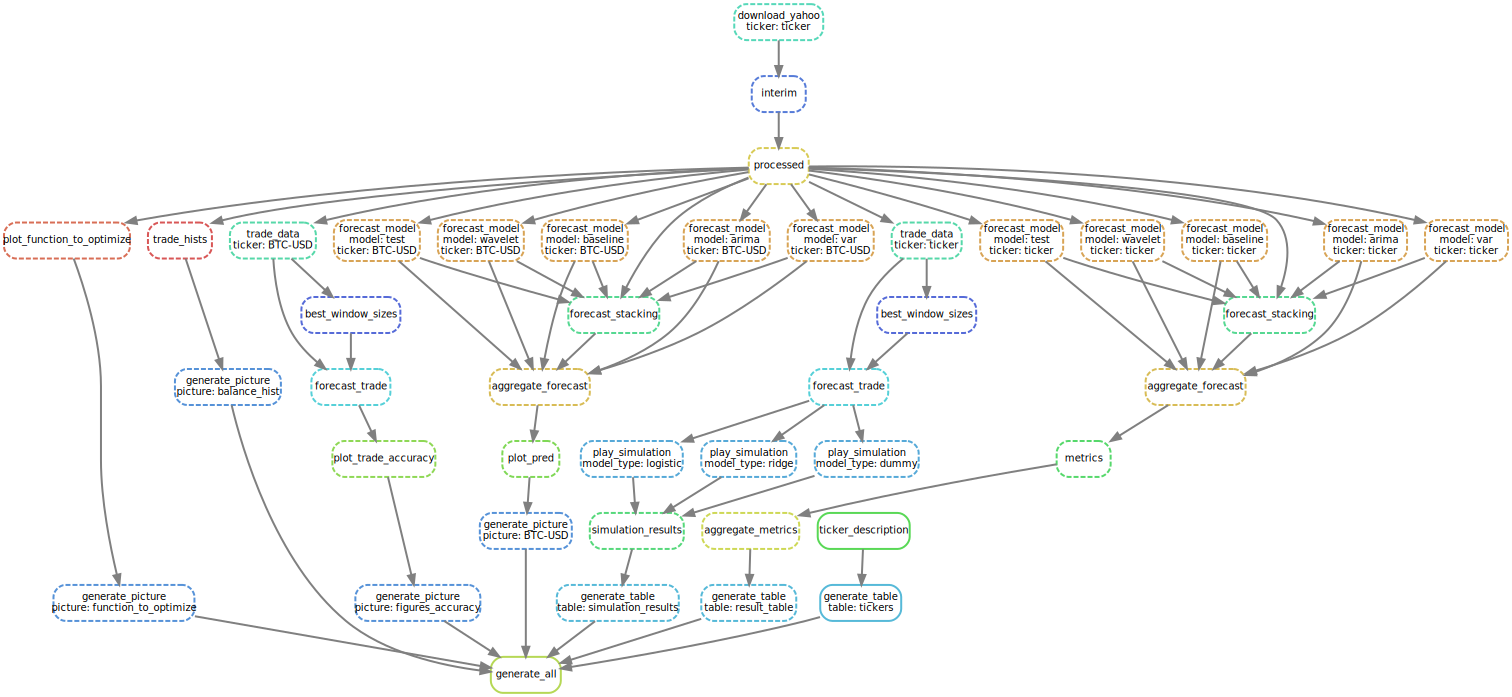
\includegraphics{../dag.svg}
}

\caption{
\label{graph_dag}
     Ациклический граф работ.}
\end {center}
\end {figure}

1.
Загружаем данные

2.
Преобразуем исходные данные в удобный формат.

3.
Используем модели для построения прогнозов по заданным датам и генерации тестовой выборки.

4.
Полученные данные используются для генерации графиков и подсчета метрик.

5.
Генерируем код LaTeX для вставки графиков и таблиц с результатами

\section{Эксперимент}

Были взяты данные с Yahoo Finance~\cite{yahoo} по акциям компаний: \textbf{написать тикеры}.
Для каждого временного ряда применялась каждая из моделей.
Модель VAR применялась сразу для всех временных рядов.
Сравнение результатов происходило по метрикам MAE, MAPE, RMSE.
Результаты можно наблюдать в таблице \textbf{ссылка на таблицу}.

\specialsection{Выводы}

Выводы

\subsection{Мотивация}

Какая-то мотивация

Ненумерованная формула:

\begin{equation}
    \begin{pmatrix} \dot{\varphi}\\ \dot{\theta} \\ \dot{\psi} \end{pmatrix}
    = \begin{pmatrix}
        cos(\theta)cos(\psi) & -sin(\psi) & 0 \\
        cos(\theta)sin(\psi) & cos(\psi)  & 0 \\
        -sin(\theta)         & 0         &  1
    \end{pmatrix}^{-1}
    \begin{pmatrix} \omega_x\\ \omega_y \\ \omega_z \end{pmatrix}.
\end{equation}

Нумерованная формула:

\begin{equation}
    i^2 = -1.
    \label{eq:my_ref}
\end{equation}

Тест ссылки на формулу ~\ref{eq:my_ref}.

Еще немного текста

\subsection{Постановка задачи}

Еще одна постановка задачи

\subsection{Доступные программные средства}

Ниже тестируется очень большая таблица на несколько страниц

\begin{center}
    \begin{longtable}{|p{2cm}|p{3cm}|p{7cm}|p{3cm}|}
    \caption{Заголовок таблицы}\\
    \hline
    1 & 2 & 3 & 4\\ 
    \hline 
    2 & 2 & 3 & 4\\
    \hline
    3 & 2 & 3 & 4\\
    \hline
    4 & 2 & 3 & 4\\
    \hline
    5 & 2 & 3 & 4\\
    \hline
    6 & 2 & 3 & 4\\
    \hline
    7 & 2 & 3 & 4\\
    \hline
    8 & 2 & 3 & 4\\
    \hline
    9 & 2 & 3 & 4\\
    \hline
    10 & 2 & 3 & 4\\
    \hline
    
    
    \end{longtable}
\end{center}


А также тестируется счетчик таблиц, жирные и двойные линии.

\begin{center}
    \begin{longtable}{|p{2cm}||p{3cm}|p{7cm}|p{3cm}|}
    \caption{Заголовок таблицы нумер 2}\\
    \hline
    1 & 2 & 3 & 4\\ 
    \hline
    2 & 2 & 3 & 4\\
    \hline
    3 & 2 & очень жирная ячейка \par с переносом (работаеттт!) & 4\\
    \hline
    4 & 2 & 3 & 4\\
    \hline
    5 & 2 & 3 & 4\\
    \hline
    6 & 2 & 3 & 4\\
    \hline
    7 & 2 & 3 & 4\\
    \hline
    8 & 2 & 3 & 4\\
    \hline
    9 & 2 & 3 & 4\\
    \hline
    10 & 2 & 3 & 4\\
    \hline
    
    
    \end{longtable}
\end{center}


\subsection{Полученные результаты}

Плейн текст

\section{Основная часть раз}

Плейн текст

\pagebreak
\section{Основная часть два: Теория}


\section{Основная часть два: Детали реализации}
\subsection{Расчётная часть}

\section{Анализ экспериментов.}
\begin{figure}[ht]
\begin{center}
\scalebox{0.4}{
   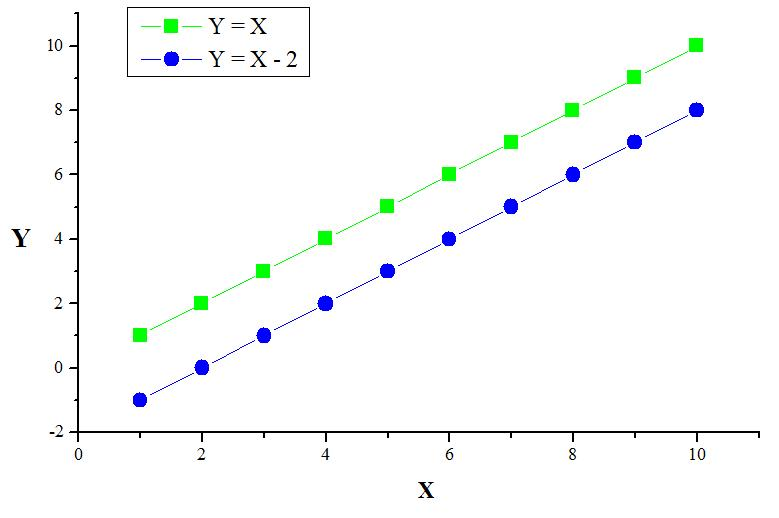
\includegraphics{images/graph.jpg}
}

\caption{
\label{graph-fig}
     Линейные функции.}
\end {center}
\end {figure}
Ссылаемся на график ~\ref{graph-fig}.
Ссылка на статью: ~\cite{voc}, ~\cite{vo2}

\specialsection{Выводы}
Жизнь --- тлен.
\pagebreak

\specialsection{Заключение}

Плейн текст

% Библиография в cpsconf стиле
% Аргумент {1} ниже включает переопределенный стиль с выравниванием слева
\begin{thebibliography}{1}
\bibitem{voc} Griffin D.W., Lim J.S. \flqq Multiband excitation vocoder\frqq. IEEE ASSP-36 (8), 1988, pp. 1223-1235.
\bibitem{vo2} Griffin D.W., Lim J.S. \flqq Multiband excitation vocoder\frqq. IEEE ASSP-36 (8), 1988, pp. 1223-1235.
\bibitem{arima} Магнус Я. Р., Катышев П. К., Пересецкий А. А. Эконометрика. Начальный курс.. М.: Дело, 2004. 576 с.
\bibitem{var} Носко В.П. Эконометрика. Введение в регрессионный анализ временных рядов
\bibitem{snakemake} Köster, Johannes and Rahmann, Sven. “Snakemake - A scalable bioinformatics workflow engine”. Bioinformatics 2012.
\bibitem{wavelet} Wang, F.; Yu, Y.; Zhang, Z.; Li, J.; Zhen, Z.; Li, K. Wavelet Decomposition and Convolutional LSTM Networks Based Improved Deep Learning Model for Solar Irradiance Forecasting. Appl. Sci. 2018, 8, 1286.
\bibitem{yahoo} https://finance.yahoo.com/
\end{thebibliography}
\end{document}